\chapter{Gray box identification}
This approach consists in defining the simplest model that can explain the real system and fit your model to experimental data collected in open loop. Therefore, we neglect every nonlinearity of the system and consider only two basic transfer functions: 
the motor
\begin{equation}
I(s) = \frac{1}{Ls+R} V(s)
\end{equation}
and the cart
\begin{equation}
X(s) = \frac{1}{Ms^2+Cs+K} F(s)
\end{equation}
connected by a constant $\gamma$ which converts the measured current into a linear force exerced onto the cart for each time instant
\begin{equation}
\gamma = \frac{2K_e}{D}=\frac{f(t)}{i(t)}
\end{equation}

The overall scheme can be drawn as follows:\\

\begin{figure}[h]
\centering
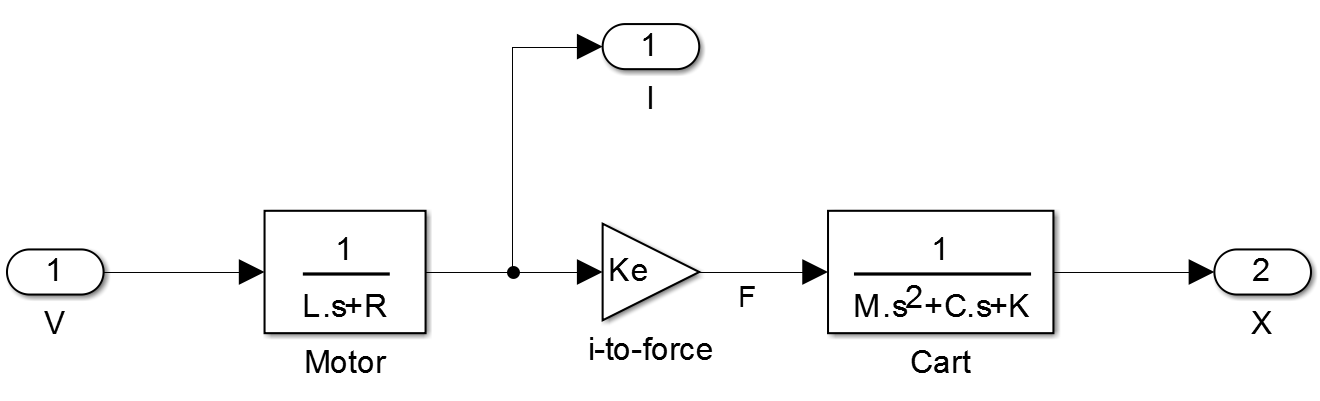
\includegraphics[width=0.6\textwidth]{img/graybox_scheme.png}
\caption{Scheme of the model employed in the identification process. The only input is the voltage applied to the motor and the accessible outputs are the measured current and the position of the cart.}
\end{figure}

In this way we are lumping all the uncertainties into 6 parameters: $L, R, \gamma, M, C, K$. This means that $C$ (for example) does not represent the damping coefficient of the spring only, but it includes all the linearised friction which is happening in the plant; the same holds for the others. Our sole interest is to derive a model which represents as close as possible the system from the perspective of the controller rather than identifying as precisely as possible the single parameters.\\

The experiment setup is very straightforward: we feed a train of pulses into the system and measure both the current and displacement of the cart; this is repeated for each spring. The pulses must be long enough to allow the cart to reach the equilibrium. Once offline, the current is filtered in order to remove the high frequency noise added by the sensor and the experiment is cut so to find the pulse window which is less noisy; this piece of data is used in the following to perform the identification.\\

The identification is performed by an optimization method. We define the measured current as $i(t)$ while the predicted one as $\hat{i}(t) = \frac{1}{Ls+R}$; the objective of the optimization is
\begin{equation}
\min_{L,R} \|i-\hat{i}\|_2^2(t)
\end{equation}
which is well known in the literature as \emph{nonlinear least squares}. Since the objective function is trivially nonlinear, we cannot guarantee the uniqueness of the minima and we need to start the optimization several times from a different set of initial condition in order to validate the results.\\

\begin{figure}[h]
\centering
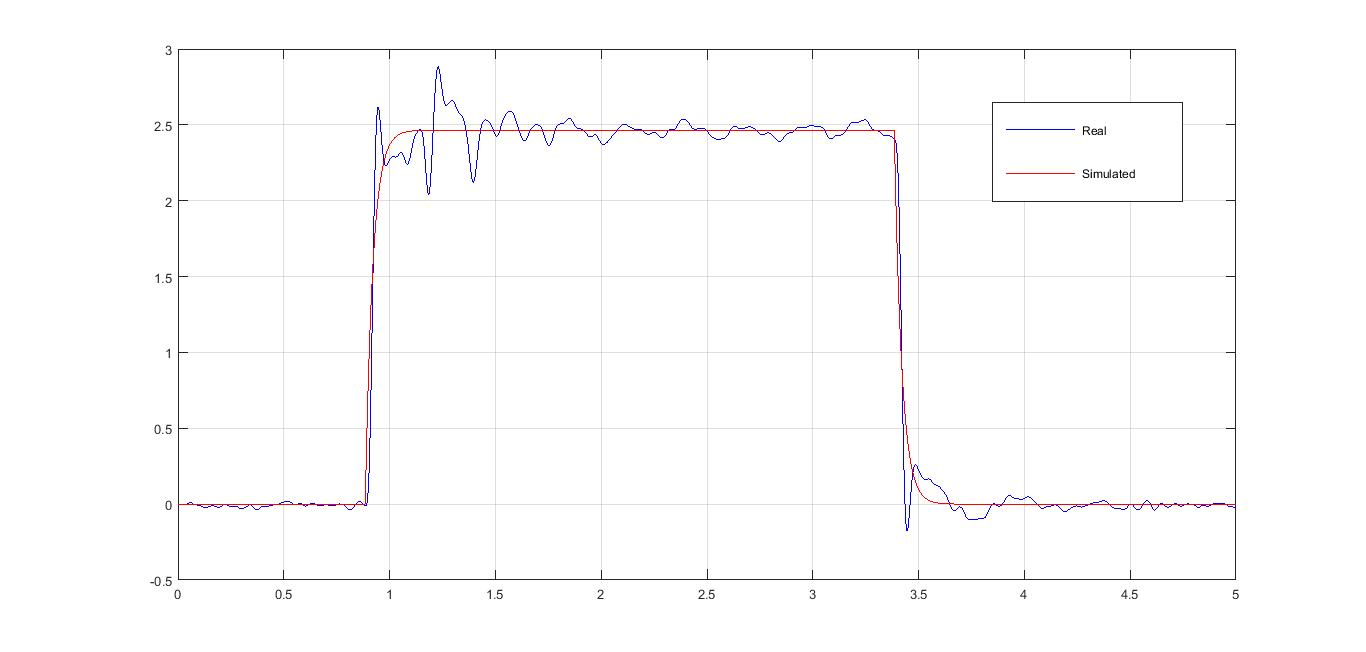
\includegraphics[width=0.35\textwidth]{img/graybox_motor.jpg}
\caption{Fitting of the model of the motor.}
\end{figure}

This process yields the following results:\\

\begin{table}[h]
\centering
\begin{tabular}{|c|c|}
R & L \\
\hline
1.3 \SI{}{\ohm}  & 0.0220 $F$ \\
\end{tabular}
\end{table}

The same applies for the identification of the cart, whilst this time we make use of the current as input and the displacement as output. Following the previous notation, the problem becomes
\begin{equation}
\min_{\gamma,M,C,K} \|x-\hat{x}\|_2^2(t)
\end{equation}
where
\begin{equation}
\hat{x}(t) = \frac{\gamma}{Ms^2+Cs+K} i(t)
\end{equation}

We can actually use either $i(t)$ or $\hat{i}(t)$ in order to have a less noisy signal as input, but the output is not very different in each case. In this scenario, the choice of the starting point of the optimization is more sensitive and needs more start than the previous and the output parameters are more variable, although the poles of the model transfer function are always the same.
\begin{figure}[h]
\centering
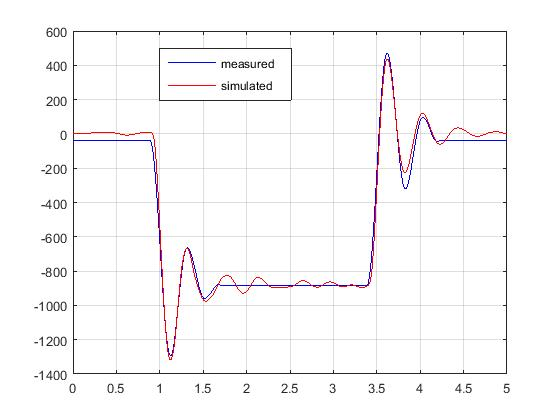
\includegraphics[width=0.35\textwidth]{img/graybox_cart.jpg}
\caption{Fitting of the model of the cart.}
\end{figure}

The identified parameters in this stage are listed below.
\begin{table}[!h]
\centering
\begin{tabular}{|c|c|c|c|c|c|c|c|}
	$\gamma$ & $M$ & $K_h$ & $K_m$ & $K_l$ & $C_h$ & $C_m$ & $C_l$ \\
	$-178.57$ $\frac{N}{A}$ & 1.3 $Kg$ & 625 $\frac{N}{m}$ & 281 $\frac{N}{m}$ & 162 $\frac{N}{m}$ & 9 $\frac{Ns}{m}$ & 6 $\frac{Ns}{m}$ & 8 $\frac{Ns}{m}$\\
\end{tabular}
\end{table}